\subsection{Alloy Model Description}
The main goal of SafeStreets is to increase safety on the strets , for reaching this goal it is importante that every report made by Citizens is taken care as fast as possible by authorities. We have modeled the goal stating that every agent must be working on an assignment if he/she is not already dealing with another. In the model there are only the entities that are relevant to this goal and semplification about users' location are made to make the model more understandable.
In addition to checking that our model with domain assumptions and requirements makes it possible to reach the goal we also checked how different worlds may be generated and that some borderline cases aren't ignored.

\subsection{Alloy Model}
\lstinputlisting[language=alloy]{Files/model.als}


\subsection{Results}
\begin{figure}[h]
\centering
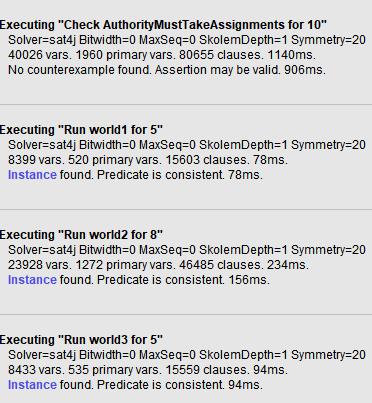
\includegraphics[width=\textwidth]{Images/alexecutionstatus.png}
\caption{Result}
\end{figure}
\begin{figure}[h]
\centering
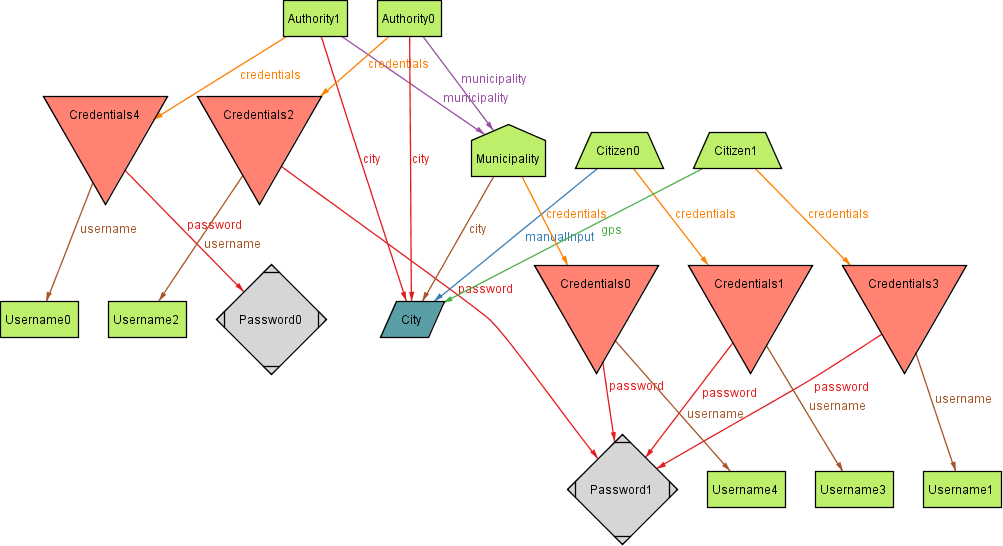
\includegraphics[width=\textwidth]{Images/alworld1.png}
\caption{First world}
\textaf{This world represents the borderline case in which no notification are present and so no assignment is associated to authorities , there are neighter statistics nor suggestions}
\end{figure}
\begin{figure}[h]
\centering
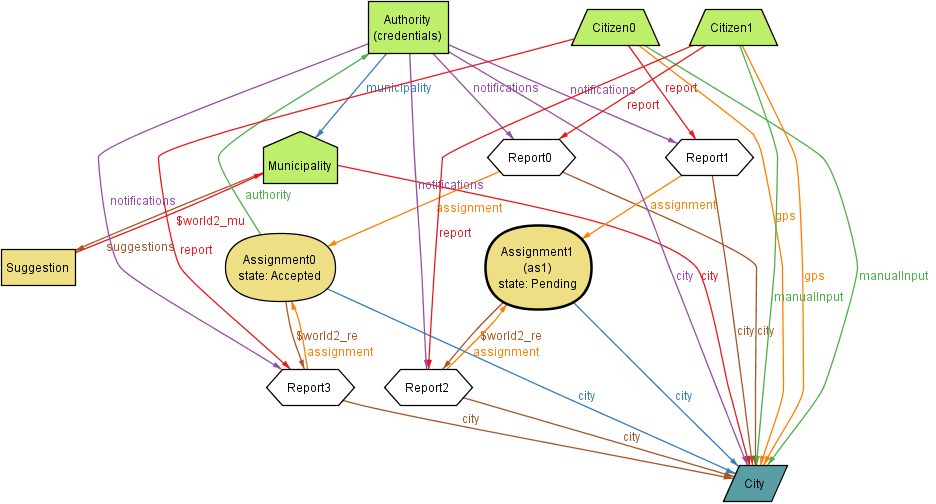
\includegraphics[width=\textwidth]{Images/alworld2.png}
\caption{Second world}
\textaf{This world represent the case in which no assignment is completed and so no statistics are available
Credentials are projected away for the sake of clarity.
}
\end{figure}
\begin{figure}[h]
\centering
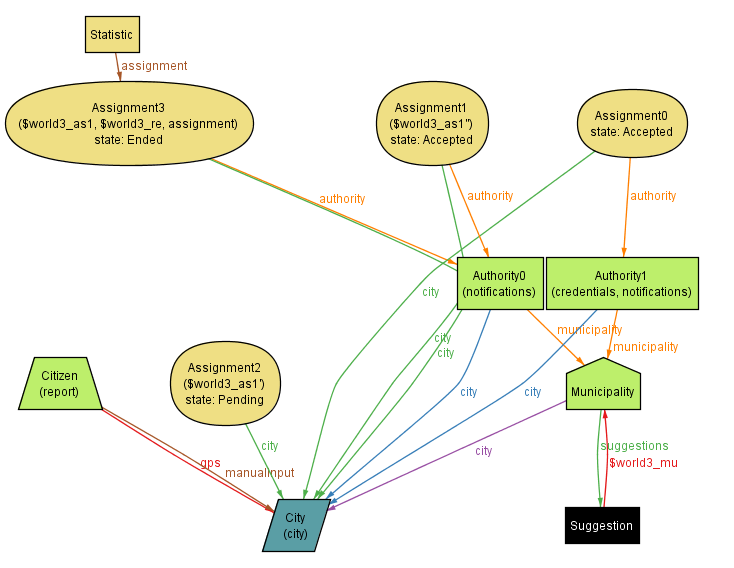
\includegraphics[width=\textwidth]{Images/alworld3.png}
\caption{Third world}
\textaf{This world represents a more generic world where assignments pending,accepted,finished are all generated.
Also here credentials are projected away for the sake of clarity.}
\end{figure}


